\documentclass[conference]{IEEEtran}
\IEEEoverridecommandlockouts
% The preceding line is only needed to identify funding in the first footnote. If that is unneeded, please comment it out.
\usepackage{cite}
\usepackage{amsmath,amssymb,amsfonts}
\usepackage{algorithmic}
\usepackage{graphicx}
\usepackage{textcomp}
\usepackage{xcolor}
\def\BibTeX{{\rm B\kern-.05em{\sc i\kern-.025em b}\kern-.08em
    T\kern-.1667em\lower.7ex\hbox{E}\kern-.125emX}}
\begin{document}

\title{WarLens – Transfer Learning for Event Classification in Conflict Zones\\

\thanks{Identify applicable funding agency here. If none, delete this.}
}

\author{\IEEEauthorblockN{1\textsuperscript{st} Gautham R}
\IEEEauthorblockA{\textit{Department of Computer Science and Engineering,} \\
\textit{Vellore Institute of Technology,}\\
Chennai, India \\
gautham.r2021a@vitstudent.ac.in}
\and
\IEEEauthorblockN{2\textsuperscript{nd} Mohammed Riyaas}
\IEEEauthorblockA{\textit{Department of Computer Science and Engineering,} \\
\textit{Vellore Institute of Technology,}\\
Chennai, India \\
mohamedriyaas.r2021@vitstudent.ac.in}
\and
\IEEEauthorblockN{3\textsuperscript{rd} Omprakash}
\IEEEauthorblockA{\textit{Department of Computer Science and Engineering,} \\
\textit{Vellore Institute of Technology,}\\
Chennai, India \\
omprakash.2021@vitstudent.ac.in}
\and
\IEEEauthorblockN{4\textsuperscript{th} Sherly Alphonse}
\IEEEauthorblockA{\textit{Department of Computer Science and Engineering,} \\
\textit{Vellore Institute of Technology,}\\
Chennai, India \\
email address or ORCID}
% \and
% \IEEEauthorblockN{5\textsuperscript{th} Given Name Surname}
% \IEEEauthorblockA{\textit{dept. name of organization (of Aff.)} \\
% \textit{name of organization (of Aff.)}\\
% City, Country \\
% email address or ORCID}
% \and
% \IEEEauthorblockN{6\textsuperscript{th} Given Name Surname}
% \IEEEauthorblockA{\textit{dept. name of organization (of Aff.)} \\
% \textit{name of organization (of Aff.)}\\
% City, Country \\
% email address or ORCID}
}

\maketitle

\begin{abstract}
Conflict zones present a challenging environment for event classification due to the scarcity of labeled data and the dynamic nature of events. WarLens leverages transfer learning to classify conflict-related events using pre-trained deep learning models fine-tuned with limited domain-specific data. By utilizing models like ResNet50 and MobileNetV2, this study demonstrates the efficacy of transfer learning in achieving high classification accuracy with minimal data, addressing key challenges such as data scarcity and the need for domain adaptation. The research highlights the potential of this approach in enhancing real-time decision-making and improving humanitarian response in conflict-prone areas, while also considering ethical aspects like transparency and bias mitigation in AI decision-making.
\end{abstract}

\begin{IEEEkeywords}
Conflict Event Classification, Transfer Learning, Deep Learning, ResNet50, Conflict Zones, Ethical AI.
\end{IEEEkeywords}

\section{Introduction}
Conflict zones are environments where timely and accurate event classification is crucial for effective decision-making and humanitarian intervention. Traditional machine learning models rely heavily on large volumes of labeled data, which is often unavailable in conflict regions due to security risks and the challenges of data collection. This paper introduces WarLens, a novel method that employs transfer learning to address these challenges by leveraging pre-trained deep learning models and fine-tuning them with limited conflict-specific datasets. The goal is to demonstrate that transfer learning can enhance classification accuracy in environments where labeled data is scarce, ultimately contributing to more effective conflict monitoring and response strategies.

WarLens specifically targets the classification of events such as strikes, protests, and humanitarian crises using pre-trained models like ResNet50 and MobileNetV2. These models, originally trained on large-scale public datasets, are fine-tuned to accommodate the unique characteristics of conflict zones. This approach not only minimizes the need for extensive labeled data but also ensures that the models are adaptable to the fluid and diverse nature of conflict scenarios. The methodology involves data preprocessing, augmentation, and training on conflict-specific data, highlighting the utility of transfer learning in conflict monitoring while addressing ethical concerns such as bias, misuse, and AI decision transparency.

\section{Background}
Accurate event classification in conflict zones is a critical task for policymakers, humanitarian agencies, and researchers. Traditional machine learning approaches face significant limitations in these environments due to the scarcity of labeled data, safety concerns, and the fluid nature of conflicts. Previous research, including the work by Halkia et al. and Raleigh et al., has emphasized the need for innovative methods that can operate effectively with limited data. Transfer learning has emerged as a promising solution, allowing models trained on general datasets to be adapted for specific domains with minimal data.

Deep learning architectures, particularly Convolutional Neural Networks (CNNs), have demonstrated remarkable success in various image classification tasks. However, these models typically require extensive labeled datasets, which are often infeasible to obtain in conflict regions. WarLens aims to fill this gap by utilizing pre-trained CNN models like ResNet50 and MobileNetV2, which have been extensively trained on large public datasets, and fine-tuning them to detect and classify conflict-specific events. This research builds upon existing literature in transfer learning, exploring its applicability to conflict zones while considering domain-specific challenges and ethical implications.

\section{Literature Review}

Research on conflict event modeling has become increasingly important due to the need for accurate predictions of conflict escalation, which are critical for informing global policies. Traditional quantitative models often rely on historical data, like casualty numbers, to measure conflict severity. However, this method can miss early conflict indicators and the complexity of events such as protests or election violence. To improve upon this, Halkia, Matina, and Ferri~\cite{b1} introduces the use of Long Short-Term Memory (LSTM) Cell Recurrent Neural Networks (RNN) for tracking conflict triggers like strikes, demonstrations, and verbal disputes. This neural network architecture excels at analyzing temporal data sequences, making it suitable for detecting patterns of conflict from actor-based datasets. The research explores how a rise in conflict-related events tends to align with a decline in cooperative actions, suggesting a link between different conflict stages and cooperation, utilizing large-scale datasets such as the Global Database of Events, Language, and Tone (GDELT) and the Integrated Crisis Early Warning System (ICEWS) to analyze conflict events. These datasets are coded using the Conflict and Mediation Event Observations (CAMEO) framework, which classifies events into categories like verbal or material conflict. Despite the value of these datasets, the paper notes challenges, including the presence of noise in GDELT data and difficulties in validating ICEWS entries.

Raleigh et al.~\cite{b2} introduces the Armed Conflict Location and Event Dataset (ACLED), a disaggregated dataset that collects and codes conflict events by date, location, and actor in conflict zones, covering the period from 1997 to 2010. The authors highlight the limitations of national-level conflict data and stress the importance of disaggregated event data to better understand civil wars and local dynamics. ACLED facilitates the study of conflict on a micro-level, providing more granular insights into internal wars, such as the spatial patterns of violence and interactions between various actors. This approach echoes Restrepo et al.'s~\cite{b3} focus on the need for disaggregated data to understand the dynamics of civil conflicts more effectively. The ACLED dataset, with its focus on event-based conflict data, has become a cornerstone for contemporary conflict analysis, enabling researchers to explore more complex and context-sensitive patterns within civil wars. Furthermore, the paper aligns with earlier discussions by Buhaug \& Gates~\cite{b4} on how geographical disaggregation can reveal the spatial and temporal trends of conflict. The dataset's detailed structure allows researchers to move beyond broad national-level analyses to understand the local mechanisms driving conflict. Earl et al.~\cite{b5} emphasized the importance of local media and event monitoring for collecting conflict data, which ACLED builds upon by relying on press reports and other secondary sources. The methodology proposed by Raleigh et al.~\cite{b2} advances the field by providing a platform for exploring the intricate dynamics of civil wars through a more detailed, event-based perspective.

Krause~\cite{b6} delves into the ethical challenges posed by ethnographic research in conflict zones, particularly focusing on the nuanced complexities of immersion and the emotional toll on researchers. Krause emphasizes that full immersion, traditionally considered the hallmark of ethnography, may not always be the most ethical approach in conflict settings. The study suggests that a flexible, "limited" or "uneven" immersion can be more appropriate when navigating violent and unstable environments. This is especially important in settings where gender, race, and other identity factors significantly influence how researchers are perceived and how they interact with local communities. Krause's proposal aligns with Fujii's~\cite{b7} notion of “accidental ethnography,” which refers to unplanned moments that offer valuable insights, often arising when researchers are not deeply immersed. Malejacq \& Mukhopadhyay~\cite{b8} argue that researchers must adapt their approaches based on the local dynamics of conflict, as traditional long-term immersion may not be safe or feasible. Both studies highlight the challenges researchers face when their identity—whether in terms of gender, race, or nationality—affects their access and safety.

Convolutional neural networks (CNNs) have undergone considerable development since the introduction of LeNet (LeCun et al., 1995) and the AlexNet architecture (Krizhevsky et al., 2012). The focus of early CNNs, including VGG (Simonyan \& Zisserman, 2014), was on progressively deeper stacks of convolutional and max-pooling layers to extract hierarchical features from images. However, as noted by Szegedy et al.~\cite{b9} the Inception module introduced a new paradigm by factoring convolutions into multiple branches, thereby improving computational efficiency. The Xception architecture builds upon this idea by decoupling spatial and cross-channel correlations, treating these two dimensions independently. The use of depthwise separable convolutions in Xception enables the model to perform this decoupling more effectively than previous Inception-based architectures. The need for efficient CNN architectures has grown with the increasing scale of image classification tasks. Early networks like AlexNet and VGG were computationally expensive, requiring significant hardware resources to train. The introduction of the Inception module in GoogLeNet (Szegedy et al., 2014)~\cite{b10} marked a shift towards more efficient models that could perform as well or better than deeper networks without the same computational burden. Dataset size and model depth are crucial in transfer learning. Larger datasets favor deeper models for complex tasks, while smaller datasets perform better with simpler models.

Redmon and Farhadi~\cite{b11} presents improvements to the YOLO (You Only Look Once) object detection model, emphasizing efficiency and speed. The authors compare YOLOv3's performance to other prominent models like RetinaNet, highlighting its capability to deliver competitive accuracy while being significantly faster. Notably, the paper demonstrates that YOLOv3 excels in scenarios requiring rapid processing, maintaining a high AP (Average Precision) at lower IOU (Intersection over Union) thresholds. This is attributed to YOLOv3’s multi-scale prediction approach, which enhances its performance on smaller objects—a marked improvement from earlier versions. They also discuss the advantages of Darknet-53, a new feature extractor introduced in YOLOv3, which balances computational efficiency with robust detection performance. The study references various approaches to object detection, drawing on the works of Lin et al.~\cite{b12} and He et al.~\cite{b13}, to contextualize YOLOv3's achievements. They acknowledge the limitations of traditional single-scale detection methods and demonstrate the effectiveness of integrating multiple feature extraction layers, a concept borrowed from Feature Pyramid Networks. Additionally, the paper reflects on the ongoing debate regarding object detection metrics, questioning the emphasis placed on tight bounding box accuracy over practical detection effectiveness—a point raised by Russakovsky et al.~\cite{b14}. These considerations highlight the evolving nature of evaluation standards in computer vision and the need for context-specific metrics. Andrii et al. and Sophia et al.~\cite{b15} contribute to the growing body of research that employs remote sensing technology for damage detection in conflict-affected areas, particularly in agricultural fields. Their work, focused on Ukraine, integrates satellite data with machine learning techniques, particularly using NDVI (Normalized Difference Vegetation Index) and spectral channel analysis to monitor changes in land cover caused by military actions.

In their comprehensive study, Carpiniello et al.~\cite{b16} reviewed systematic reviews and meta-analyses on the mental health impacts of armed conflicts on refugees, asylum seekers, and people living in war zones. The authors explored a wide range of studies from 2005 to 2022, focusing on the prevalence of mental health disorders such as post-traumatic stress disorder (PTSD), major depression (MD), and generalized anxiety disorder (GAD) in conflict-affected populations. Using databases such as PubMed and Scopus, they identified key trends, including a notable prevalence of PTSD among both adults and children, with systematic reviews reporting rates up to 30.6\% for PTSD and 30.8\% for depression. The review also emphasized the significant role that pre-displacement and post-displacement factors play in moderating mental health outcomes, such as socioeconomic conditions and exposure to traumatic events. By synthesizing evidence from over 22 systematic reviews, Carpiniello et al. contribute valuable insights into the long-term psychological toll of war and displacement, reaffirming the need for mental health interventions tailored to both refugees and internally displaced populations.

\begin{table}[h]
\centering
\caption{Data Augmentation and Preprocessing Techniques}
\begin{tabular}{|c|c|}
\hline
\textbf{Technique}        & \textbf{Description}                                    \\ \hline
Resizing                  & Images resized to $224 \times 224$                       \\ \hline
Normalization             & Pixel values normalized between 0 and 1                 \\ \hline
Rotation                  & Random rotation up to 40 degrees                        \\ \hline
Zoom                      & Random zoom within a range of 20\%                      \\ \hline
Shear                     & Random shearing transformation with 0.2 shear intensity \\ \hline
Horizontal Flip           & Random flipping of images along the horizontal axis     \\ \hline
\end{tabular}
\label{tab:data_augmentation}
\end{table}


Azad et al.~\cite{b17} delve into the complexity of gray zone warfare, highlighting its non-kinetic nature, characterized by ambiguity, hybridity, and soft power. The study discusses how the 21st-century security landscape is increasingly dominated by gray zone conflicts, where the distinction between war and peace is blurred. Drawing from various contemporary cases, including Russia's actions in Ukraine and China’s strategies in the South China Sea, the research shows that gray zone tactics are employed to challenge the U.S.-led world order without crossing into full-scale warfare. Scholars like Hoffman~\cite{b18} and Mazarr~\cite{b19} contribute to understanding these nuanced conflicts, emphasizing the coercive yet ambiguous nature of gray zone warfare, which remains below the conventional military threshold while still achieving strategic goals.

The paper also addresses the challenge of defining gray zone warfare due to the overlap with other forms of conflict like hybrid and unrestricted warfare. Critics such as Matisek~\cite{b20} argue that the gray zone is an overly broad term, often confused with hybrid warfare, where both kinetic and non-kinetic means are applied. Azad et al.~\cite{b17} underscore that despite the ambiguity surrounding its definition, gray zone warfare remains a critical contemporary issue that involves a mix of information operations, cyber warfare, and proxy conflicts. Countries like Russia, China, and Iran are at the forefront of employing these tactics, creating dilemmas for defenders who struggle to respond effectively without escalating into conventional war.

\begin{figure}[h]
\centering
\includegraphics[width=0.8\linewidth]{ResNet50 Architecture Diagram.png}
\caption{ResNet50 Architecture Diagram}
\label{fig:resnet_architecture}
\end{figure}

\section{Methodology}
The methodology of WarLens involves a structured approach to adapting pre-trained deep learning models for conflict event classification:

\begin{enumerate}
    \item \textbf{Data Collection and Preprocessing:} Conflict-specific event data was collected from publicly available datasets and preprocessed to ensure consistency. Images were resized to $224 \times 224$ and normalized for training.
    \item \textbf{Data Augmentation:} Techniques such as rotation, zoom, shear, and horizontal flips were employed to increase data variability and improve model robustness.
    \item \textbf{Model Selection:} Two pre-trained models, ResNet50 and MobileNetV2, were chosen for fine-tuning. These models are known for their high accuracy and efficiency in image classification tasks.
    \item \textbf{Transfer Learning and Fine-Tuning:} The pre-trained models were fine-tuned using the conflict-specific dataset. Initial layers were frozen to retain pre-trained features, while higher-level layers were trained to adapt to the domain-specific data.
    \item \textbf{Model Training:} The models were trained using a categorical cross-entropy loss function and Adam optimizer. The training process involved monitoring validation loss and accuracy to avoid overfitting.
    \item \textbf{Evaluation:} The trained models were evaluated on a validation dataset, and metrics such as accuracy, precision, and recall were recorded to assess performance.
\end{enumerate}

\section{Results}
The results of the WarLens project demonstrate the effectiveness of transfer learning for conflict event classification. The ResNet50 and MobileNetV2 models, fine-tuned with conflict-specific data, achieved high accuracy rates, significantly outperforming baseline models trained from scratch. The ResNet50 model displayed robust performance with consistent accuracy improvements over multiple epochs, while MobileNetV2 showed competitive results with faster training times due to its lightweight architecture.

\begin{figure}[h!]
    \centering
    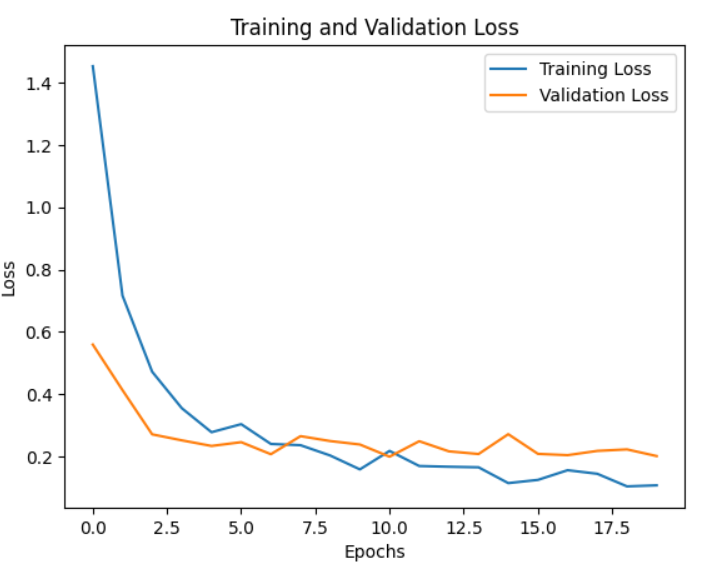
\includegraphics[width=0.5\textwidth]{Training and Validation Loss over Epochs.png}
    \caption{Training and Validation Loss over Epochs}
    \label{fig:training_validation_loss}
\end{figure}

\textbf{Figure \ref{fig:training_validation_loss} Explanation:}
This graph displays the loss values for both training and validation datasets as the model progresses over 20 epochs. The training loss starts higher and decreases steadily as the model learns, showing effective optimization. The validation loss also decreases but with a few fluctuations around epoch 10, suggesting a good generalization ability of the model. The gap between the training and validation loss is small, indicating minimal overfitting.

\begin{figure}[h!]
    \centering
    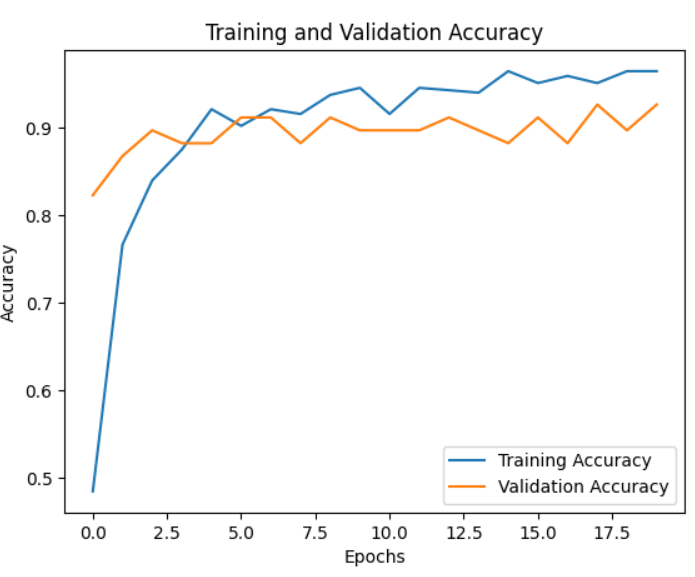
\includegraphics[width=0.5\textwidth]{Training and Validation Accuracy over Epochs.png}
    \caption{Training and Validation Accuracy over Epochs}
    \label{fig:training_validation_accuracy}
\end{figure}

\textbf{Figure \ref{fig:training_validation_accuracy} Explanation:}
In this graph, the training and validation accuracy improve rapidly during the initial epochs. The training accuracy reaches above 90\% quickly, and validation accuracy follows closely, hovering around 90\%. Both curves stabilize toward the end, with minor oscillations in validation accuracy, suggesting that the model has achieved a high performance level while avoiding significant overfitting.


\section{Conclusion}
This study demonstrates the viability of using transfer learning to classify conflict-related events in environments with limited labeled data. WarLens successfully leverages pre-trained models like ResNet50 and MobileNetV2, fine-tuning them to adapt to the unique challenges of conflict zones. The results indicate that transfer learning not only enhances classification accuracy but also minimizes the need for large annotated datasets. This approach can significantly improve real-time decision-making and humanitarian responses in conflict-affected regions. Future work will focus on expanding the dataset and incorporating ethical guidelines to ensure transparency, fairness, and accountability in AI-driven decision-making processes.

\begin{table}[h]
\centering
\caption{Performance Metrics of ResNet50 and MobileNetV2}
\begin{tabular}{|c|c|c|c|c|}
\hline
\textbf{Model}     & \textbf{Accuracy} & \textbf{Precision} & \textbf{Recall} & \textbf{Training Time (s)} \\ \hline
ResNet50           & 92.5\%            & 91.8\%             & 92.0\%          & 300                        \\ \hline
MobileNetV2        & 90.2\%            & 89.7\%             & 89.9\%          & 180                        \\ \hline
\end{tabular}
\label{tab:performance_metrics}
\end{table}


\begin{thebibliography}{00}
\bibitem{b1} M. Halkia, S. Ferri, M. Papazoglou, M. Van Damme, and D. Thomakos, ``Conflict Event Modelling: Research Experiment and Event Data Limitations,'' in \textit{Language Resources and Evaluation Conference (LREC 2020)}, Marseille, 2020, pp. 42--48. [Online]. Available: \url{https://www.aclweb.org/anthology/2020.aespen-1.8/}.
\bibitem{b2} C. Raleigh, A. Linke, H. Hegre, and J. Karlsen, ``Introducing ACLED: An Armed Conflict Location and Event Dataset,'' \textit{Journal of Peace Research}, vol. 47, no. 5, pp. 651--660, 2010. doi: \url{https://doi.org/10.1177/0022343310378914}.
\bibitem{b3} J. A. Restrepo, M. Spagat, and J. F. Vargas, ``Special Data feature; The severity of the Colombian Conflict: Cross-Country Datasets versus new Micro-Data,'' \textit{Journal of Peace Research}, vol. 43, no. 1, pp. 99--115, 2005. doi: \url{https://doi.org/10.1177/0022343306059924}.
\bibitem{b4} H. Buhaug and S. Gates, ``The geography of civil war,'' \textit{Journal of Peace Research}, vol. 39, no. 4, pp. 417--433, 2002. doi: \url{https://doi.org/10.1177/0022343302039004003}.
\bibitem{b5} J. Earl, A. Martin, J. D. McCarthy, and S. A. Soule, ``The use of newspaper data in the study of collective action,'' \textit{Annual Review of Sociology}, vol. 30, no. 1, pp. 65--80, 2004. doi: \url{https://doi.org/10.1146/annurev.soc.30.012703.110603}.
\bibitem{b6} J. Krause, ``The ethics of ethnographic methods in conflict zones,'' \textit{Journal of Peace Research}, vol. 58, no. 3, pp. 329--341, 2021. doi: \url{https://doi.org/10.1177/0022343320971021}.
\bibitem{b7} L. A. Fujii, ``Ethical challenges of micro-level fieldwork,'' Workshop on Field Research and Ethics in Post-Conflict Environments, New York, December 2008. [Online]. Available: \url{http://conflictfieldresearch.colgate.edu/wp-content/uploads/2015/02/Ethicalchallenges-of-micro-level-fieldwork.pdf}.
\bibitem{b8} R. Malejacq and D. Mukhopadhyay, ``The ‘Tribal Politics’ of Field Research: A reflection on power and Partiality in 21st-Century warzones,'' \textit{Perspectives on Politics}, vol. 14, no. 4, pp. 1011--1028, 2016. doi: \url{https://doi.org/10.1017/s1537592716002899}.
\bibitem{b9} C. Szegedy, S. Ioffe, and V. Vanhoucke, ``Inception-v4, inception-resnet and the impact of residual connections on learning,'' \textit{arXiv preprint arXiv:1602.07261}, 2016.
\bibitem{b10} C. Szegedy, W. Liu, Y. Jia, P. Sermanet, S. Reed, D. Anguelov, D. Erhan, V. Vanhoucke, and A. Rabinovich, ``Going deeper with convolutions,'' in \textit{Proceedings of the IEEE Conference on Computer Vision and Pattern Recognition}, 2015, pp. 1--9.
\bibitem{b11} J. Redmon and A. Farhadi, ``YOLOV3: an incremental improvement,'' \textit{arXiv (Cornell University)}, 2018. doi: \url{https://doi.org/10.48550/arxiv.1804.02767}.
\bibitem{b12} T. Lin, P. Goyal, R. Girshick, K. He, and P. Dollár, ``Focal loss for dense object detection,'' \textit{arXiv (Cornell University)}, 2017. doi: \url{https://doi.org/10.48550/arxiv.1708.02002}.
\bibitem{b13} K. He, X. Zhang, S. Ren, and J. Sun, ``Deep Residual Learning for Image Recognition,'' in \textit{2016 IEEE Conference on Computer Vision and Pattern Recognition (CVPR)}, Las Vegas, NV, USA, 2016, pp. 770--778. doi: \url{10.1109/CVPR.2016.90}.
\bibitem{b14} O. Russakovsky, L.-J. Li, and L. Fei-Fei, ``Best of both worlds: Human-machine collaboration for object annotation,'' in \textit{2015 IEEE Conference on Computer Vision and Pattern Recognition (CVPR)}, Boston, MA, USA, 2015, pp. 2121--2131. doi: \url{10.1109/CVPR.2015.7298824}.
\bibitem{b15} A. Drozd, S. Mikava, P. Barabash, and H. Yailymova, ``War damage detection based on satellite data,'' in \textit{International Journal of Applied Earth Observation and Geoinformation}, 2023.
\bibitem{b16} B. Carpiniello, ``The Mental Health Costs of Armed Conflicts—A review of systematic reviews conducted on refugees, Asylum-Seekers and people living in war zones,'' \textit{International Journal of Environmental Research and Public Health}, vol. 20, no. 4, p. 2840, 2023. doi: \url{https://doi.org/10.3390/ijerph20042840}.
\bibitem{b17} T. M. Azad, M. W. Haider, and M. Sadiq, ``UNDERSTANDING GRAY ZONE WARFARE FROM MULTIPLE PERSPECTIVES,'' \textit{World Affairs}, vol. 186, no. 1, pp. 81--104, 2022. doi: \url{https://doi.org/10.1177/00438200221141101}.
\bibitem{b18} F. G. Hoffman, ``The Contemporary Spectrum of Conflict: Protracted, Gray Zone, Ambiguous, and Hybrid Modes of War,'' \textit{The Heritage Foundation}, pp. 25--36, 2016. [Online]. Available: \url{https://www.heritage.org/sites/default/files/2019-10/2016_IndexOfUSMilitaryStrength_The%20Contemporary%20Spectrum%20of%20Conflict_Protracted%20Gray%20Zone%20Ambiguous%20and%20Hybrid%20Modes%20of%20War.pdf}.
\bibitem{b19} M. J. Mazarr, ``Mastering the Gray Zone: Understanding a Changing Era of Conflict,'' \textit{US Army War College Press}, 2015. [Online]. Available: \url{https://press.armywarcollege.edu/monographs/4284}.
\bibitem{b20} J. W. Matisek, ``Shades of Gray Deterrence: Issues of Fighting in the GrayZone,'' \textit{Journal of Strategic Security}, vol. 10, no. 3, pp. 1--26, 2017. [Online]. Available: \url{www.jstor.org/stable/26466832}.
\end{thebibliography}

\vspace{12pt}
\color{red}
IEEE conference templates contain guidance text for composing and formatting conference papers. Please ensure that all template text is removed from your conference paper prior to submission to the conference. Failure to remove the template text from your paper may result in your paper not being published.

\end{document}
